\chapter{Results}
\label{ch:results}

\emph{In this chapter the results of the experiments and methods detailed in the methodology chapter \Sref{ch:methodology} and background chapter \Sref{ch:background} are presented.}
\emph{A detailed analysis of the results is included along with references to similar results within the literature.}
\emph{Both quantitative and qualitative analysis is carried out and the limitations of the metrics used are discussed.}

\emph{First, the reproduction of {\scshape Steering Clear} \citep{steering-clear} detailed in \Sref{sec:steering-clear} is presented.}
\emph{Comparisons to the original paper are made along with additional analysis.}
\emph{This provides hypotheses about how the same adaptors will behave in the natural language setting of LLMs \Sref{sec:prompt-pairs}.}

\emph{Finally, the natural language setting described in the methodology chapter \Sref{sec:prompt-pairs} is analysed.}
\emph{A comparison to the {\scshape Steering Clear} toy environment is made focusing on the hypotheses proposed.}
\emph{Additionally, an in depth analysis of the hyperparameter choice in comparison to the toy environment is carried out.}
\emph{This provides potential further avenues of research and implications of superposition \Sref{sec:sae} on steering adaptors.}

\section{{\scshape Steering Clear} Reproduction}
\label{sec:steering-clear-res}

The results of the reproduction suggest that the analysis by \citet{steering-clear} are sound though an exact replication was not achieved.

\begin{figure}
    \centering
    \captionsetup{width=\textwidth}
    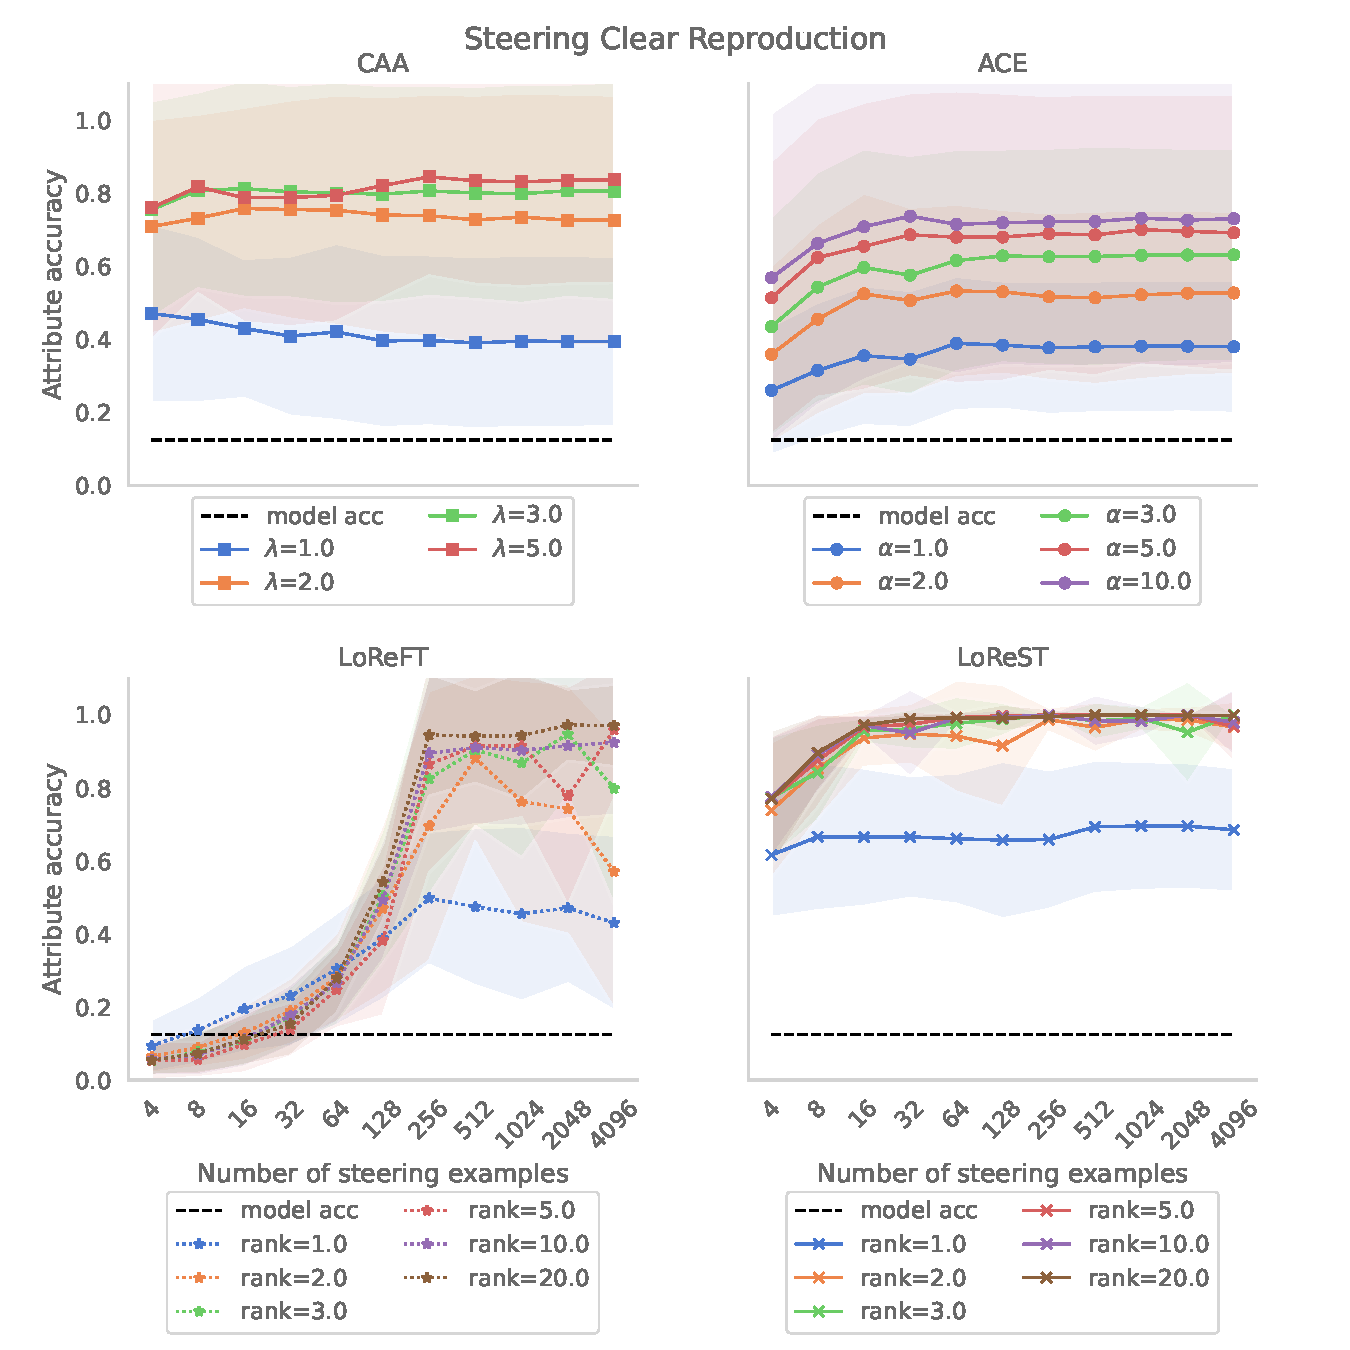
\includegraphics[width=\textwidth]{figures/steering_clear.pdf}
    \caption{
        The average accuracy of the steered model predicting the correct attribute value, in all cases this is $\mu_1$ (see \Sref{sec:steering-clear}).
        This represents how well the adaptor was able to steer the models output towards the correct value for the given attribute.
        In contrast to Figure 1 in \citet{steering-clear} only the target attribute is considered in comparison to all attributes.
        The same trends of consistent performance for affine methods and a clear increase in performance for low-rank methods are present as in \citet{steering-clear}.
    }
    \label{fig:steering-clear}
\end{figure}

The results of \cite{steering-clear} are reproduced in \Fref{fig:steering-clear} following the experimental setup in \Sref{sec:steering-clear}.
There are a few changes from Figure 1 in \cite{steering-clear}, primarily the steering metric focuses on the steered attribute rather than entire output label.
Furthermore, ACE is added and minimally modified counterfactuals (MiMiC) \citep{mimic} is removed.
A full discussion of the different metric and why this was used is presented in \Aref{app:steering-clear}.

The figure clearly shows a difference between the linear/affine methods of CAA \& ACE and the low-rank methods of LoReFT \& LoReST.
In the limit of more examples both low-rank methods achieve near 100\% success rate in steering the target attribute to the target value.
In comparison the affine methods reach an asymptote ($\sim 0.8$ for most hyperparameters) which does not increase with more training examples.
Importantly, in the low training example setting both LoReFT performs worse than both CAA and ACE.
In fact, it performs worse than the model without steering.
This is due to the requirement to train parameters which both affine approaches lack.
However, the addition of parameters allows the method to perform better as more examples are presented.
This feature of improvement with more examples is shared with LoReST.

Across the methods there is a critical hyperparameter value above which the adaptors performance does not significantly improve.
In the case of CAA this appears to be $\lambda=2$; for LoReFT the threshold rank is likely 3 as 2 decreases in accuracy as more examples are introduced; finally with LoReST the rank is clearly 2.
ACE behaves differently due to it's design (detailed in \Sref{sec:ace}) where the parameters relate to the strength of the behaviour more directly.
This is visible in \Fref{fig:steering-clear} as clear bands as the hyperparameter increases; in comparison to the other plots where after a threshold hyperparameter value the adaptors behave similarly.

Similar to the findings of \citet{steering-clear} LoReFT plateaus after 256 examples which coincides with the dimension of the activation space.
This distinction is not present in the other methods though this is similar to the Figure in \citet{steering-clear}.
A possible explanation for this in the case of the affine methods is they do not learn their own representation.
Instead, with sufficient opposing examples, the difference in steering direction is minimal with more examples.

LoReST in comparison to both LoReFT and the affine methods incorporates both affine steering and low-rank steering.
This means in the low data regime it behaves closer to ACE and CAA relying on the bias term; when enough data is provided LoReST can encode the concepts sufficiently resulting in an increase in accuracy.
This is supported by the fact that LoReST achieves an accuracy of $\sim 0.8$ with 4 examples matching CAA, and then LoReST then continues to increase in accuracy eventually plateauing at the same accuracy as LoReFT, $\sim 1.0$.
This behaviour matches those presented in \citet{steering-clear}.

\section{Prompt Pairs}
\label{sec:prompt-pairs-res}

\subsection{Quantitative Analysis}
\label{sec:quant}

Recall the three metrics defined in \Sref{sec:prompt-pairs} of target SAE feature activation, spurious SAE feature activation and semantic similarity.
As there is no notion of accuracy akin to \citet{steering-clear} the closest comparison comes from the activation of SAE features.
To avoid indiscriminate increase across all SAE features, the spurious SAE features verifies the model only affects the target concepts.

\subsubsection{SAE Target Feature Activation}

\begin{figure}
    \centering
    \captionsetup{width=\textwidth}
    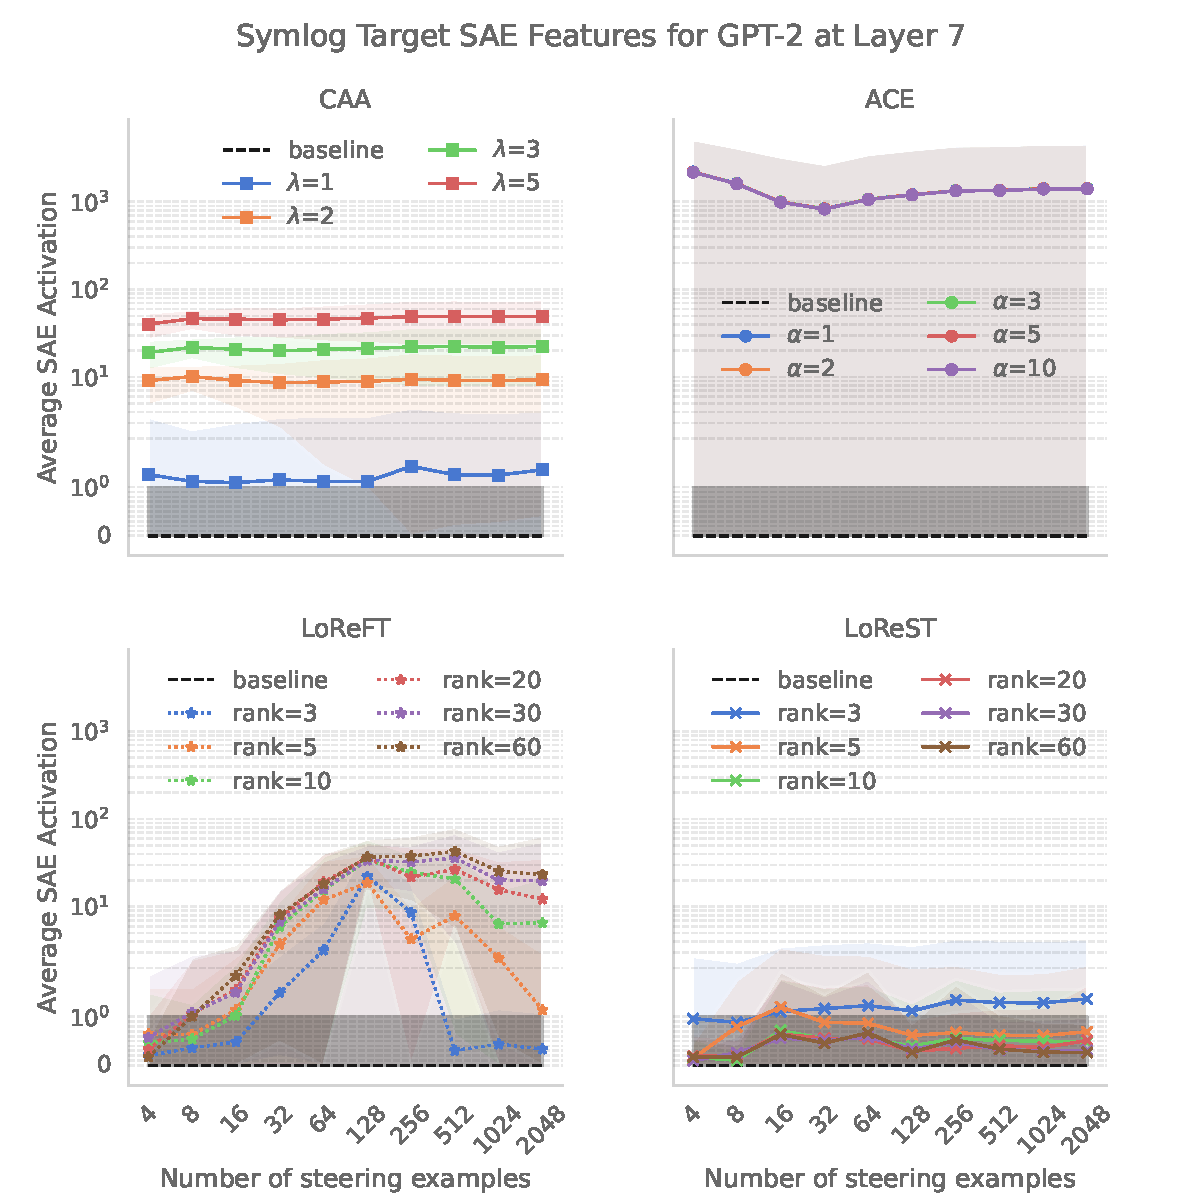
\includegraphics[width=\textwidth]{figures/gpt2_7_target.pdf}
    \caption{
        The average activation of target SAE features at the model completion tokens.
        This represents how well the adaptor positively changed the models representation, \emph{higher} values are better.
        The y axis is a symmetric logarithm scale where the range $[0,1]$ is linear, this section is highlighted in grey.
        The same range of examples is used across all adaptors.
    }
    \label{fig:gpt-pp-target}
\end{figure}

\Fref{fig:gpt-pp-target} presents the results of the first metric, the average activation of the target SAE features.
As discussed in \Sref{sec:prompt-pairs} the target SAE features are the SAE features that had the highest, average activation across all positive examples.
For this reason, a successful adaptor should increase the activation of these SAE features from the model with no intervention.

The figure uses a symmetric logarithmic scale where the range -1 to 1 is linear and all other regions are logarithmic.
The symmetric logarithmic scale is used as the activations range from 0 exponentially up to 1000 and 0 is not representable on a standard logarithmic scale.
The linear region of the plot is highlighted in gray and a horizontal grid is provided to demonstrate the difference.

From the figure most methods provide some level of improvement regardless of hyperparameter choice, however, LoReST does not provide a significant improvement compared to the others.
However, the results presented do not match those those of \citet{steering-clear} where low-rank methods consistently outperform affine methods.
This demonstrates that though useful insight is gained from the toy setup of \textsc{Steering Clear} this does not lead to predictable results in the natural language setting.
The primary outliers are ACE and LoReST.

\smalltitle{CAA} matches the behaviour in the steering clear environment \Sref{sec:steering-clear}.
There is a clear increase in effectiveness as the steering magnitude $\lambda$ increases and the performance is constant across the number examples with minor fluctuations.

In the case of $\lambda = 5$ the adaptor achieves an average SAE activation of $46.7 \pm 7.8$ across the range of training examples.
In the case of $\lambda = 1$ the adaptor achieves an average of $1.2 \pm 0.01$.
This demonstrates a very consistent value across the number of examples regardless of hyperparameter.
However, the larger the parameter the greater the variance in the exact SAE feature activation.

In comparison to CAA in \citet{steering-clear}, presented in \Fref{fig:steering-clear}, the same behaviour is observed.
A consistent value across the number of steering examples with a clear threshold above $\lambda = 1$.
This suggests that in unseen examples the CAA adaptor has to overcompensate and perturb the representation further in representation space than what was learnt.

\smalltitle{ACE} does not behave as expected or in line with the findings presented in \Sref{sec:steering-clear-res}.
The hyperparameter does not change the target activation significantly and across trained examples the average activation value decreases.
The method, however, has the highest average target activation by an order of magnitude compared to the next best adaptor.
This is accompanied by the largest variance across the adaptors, at its best ACE achieves a feature activation of $2187$ but has a standard deviation of $2912$.
This variance is consistent across the range of training examples.
The problem of variability across all the adaptors is discussed further in \Sref{sec:variability}.

Given that \citet{ace} demonstrate impressive performance of ACE on Llama 3 \citep{llama3} and the comparable performance of ACE and CAA in \Fref{fig:steering-clear} it is likely that the task, the model or the metric are ill suited to the adaptor.
The emergent properties present in larger models such as Llama 3 \citep{llama3} and GPT 5 \citep{gpt-5} are not as prominent in the smaller GPT 2 \citep{gpt-2} model.
It is possible that across positive and negative examples there is not a clear, meaningful baseline from which ACE can consistently steer from.
This could be due to the completions involving free-text answers that have a range of interpretations that may not align with the desired interpretation.

\smalltitle{LoReFT} behaves according to \citet{steering-clear}.
In particular there is a clear increase in target feature activation as the number of examples increases until a threshold point from which the adaptor does not improve.

In the majority of hyperparameter choices the best performance occurred between 128 and 512 examples.
This does not line up with the predictions of \citet{steering-clear} who found that the point of best performance occurred when the number of examples matched the activation dimension.
In \Fref{fig:gpt-pp-target} the activation dimension of GPT-2 is 756 \citep{saelens} compared to the optimal performance occurring at 128-512 examples.

The key differences between the toy setup and this environment is the added complexity of superposition \Sref{sec:sae}.
However, this would suggest that superposition \emph{decreases} the number of required examples to successfully steer.
Another possibility is the rank of the adaptor is too small to accurately steer the model.
This is supported by the fact that the average feature activation decreases rather than plateaus similar to the small rank examples in \Fref{fig:steering-clear} (see $rank=1, 2$).

LoReFT at its optimal is comparable to CAA achieving an average feature activation of $42.8 \pm 37.2$ in comparison to CAA with $49.3 \pm 26.3$.
However, in comparison to CAA, LoReFT requires careful tuning of the hyperparameter and the number of examples provided.
This behaviour is seen both in this realistic environment and the toy environment \Sref{sec:steering-clear-res}.

\smalltitle{LoReST} does not follow the trend presented in \citet{steering-clear}.
In comparison to \Fref{fig:steering-clear} there is no clear increase in the chosen metric as the number of examples increase.
Furthermore, the optimal rank appears to be $3$ rather than the larger ranks as anticipated.
Even the optimal rank of $3$ appears to perform worse that CAA with LoReST's average of $1.17 \pm 0.03$ compared to $1.21 \pm 0.01$ for CAA.

From \Fref{fig:steering-clear} it may be expected that the exact rank of LoReST has limited effect on the performance of the adaptor.
However, the results in \Fref{fig:steering-clear} suggest that there is a hyperparameter threshold above which the adaptor performs similarly \emph{but} higher values are not necessarily better.

\begin{figure}
    \centering
    \captionsetup{width=\textwidth}
    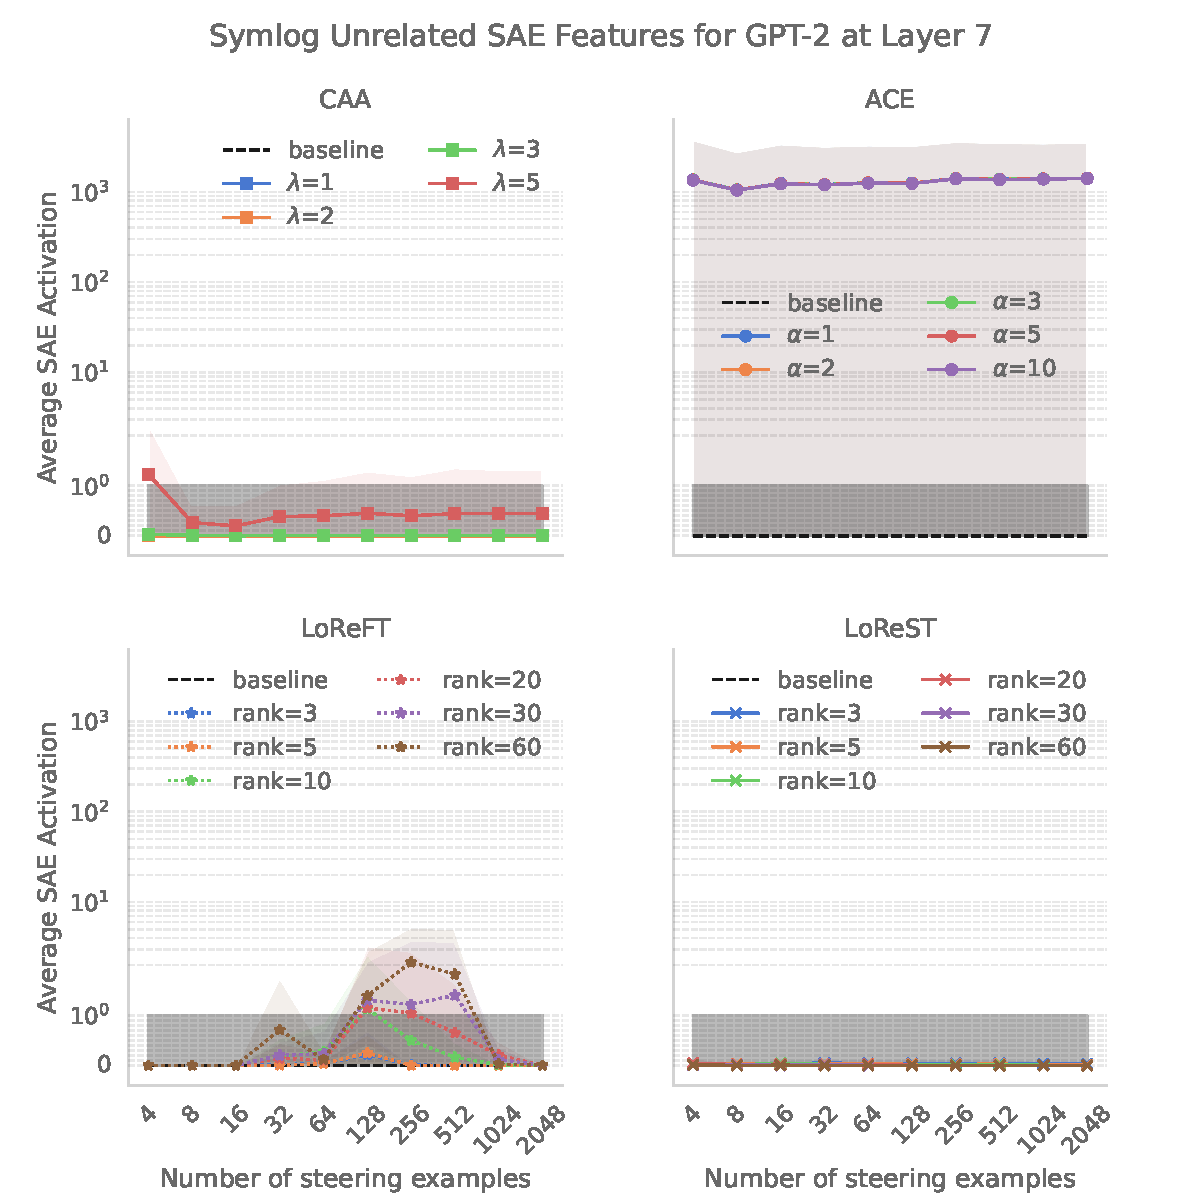
\includegraphics[width=\textwidth]{figures/gpt2_7_unrelated.pdf}
    \caption{
        The average activation of unrelated SAE features at the model completion tokens.
        This represents how well the adaptor did not interfere, \emph{lower} values are better.
        The y axis is a symmetric logarithm scale where the range $[0,1]$ is linear, this section is highlighted in grey.
        This demonstrates that all but ACE achieve 0 interference in some instances.
        The same range of examples is used across all adaptors.
    }
    \label{fig:gpt-pp-unrelated}
\end{figure}

Unlike the other adaptors presented here LoReST has not be thoroughly applied to large language models (LLMs).
It is possible that this approach, though based on adaptors such as LoReFT, is not suitable.
\emph{However}, as demonstrated in both \Fref{fig:gpt-pp-unrelated} and \Sref{sec:qual} the seemingly poor performance of LoReST suggests that feature activation alone is a poor metric for assessing success of a steering adaptor.

\subsubsection{SAE Spurious Feature Activation}

\Fref{fig:gpt-pp-unrelated} presents the results of the second metric, the average activation of the spurious SAE features.
As discussed in \Sref{sec:prompt-pairs} the spurious SAE features are the SAE features that where not activated in either the positive or negative examples.
These features represent concepts that are, in theory, unrelated to concepts represented across the example prompts.
Only a random sample is considered rather than the entirety of spurious features which is usually fairly large.
For this reason, a successful adaptor should not activate any of these features resulting in an average of 0, in general a low or decreasing average activation is expected.

Following \Fref{fig:gpt-pp-target} the figure uses a symmetric log plot with the same linear region highlighted.
This is particularly important in this case as the majority of values are expected to be 0, however certain adaptors can result in very large activations.
The same scale as \Fref{fig:gpt-pp-target} is used for comparison.

Comparing against \Fref{fig:gpt-pp-target}, \Fref{fig:gpt-pp-unrelated} demonstrates a different set of benefits to each of the adaptors.
In particular, the two figures show the trade offs between high target feature activation and low spurious feature activation.
From this plot it is clear to see how well LoReST is able to accurately manipulate the models internal representations.

\smalltitle{CAA} performs very well considering both metrics.
The adaptor is able to increase the target SAE feature activation whilst maintaining a suitably low spurious feature activation.
This suggests that the adaptor is able to precisely manipulate the internal representation along the desired concept.

As stated previously it achieves a target feature activation of up to $49.3$ but also has a maximum spurious feature activation of $0.45 \pm 0.87$ when $\lambda = 5$.
In the case of $\lambda = 3$ the target feature activation is $22.3 \pm 14.6$ with spurious feature activation $0.0012 \pm 0.0002$.
As with the target feature activation there is still a substantial amount of variance in the spurious feature activation.

The large spurious feature activation for $\lambda = 5$ in comparison to the other hyperparameters can be attributed to the linear nature of the adaptor.
When the steering vector magnitude is too large it is likely to push the representation outside of the desired representation space.
This can have unintended consequences as shown here, where other concepts that were not intended are boosted.
For this reason it is expected for affine methods to perform worse than low rank methods that can perform more complex manipulations.

\smalltitle{ACE} demonstrates further problems as it maintains a high activation for spurious features.
Similar to \Fref{fig:gpt-pp-target} there is a high variance in the activation.
Together these plots demonstrate a high level of inconsistency across the different datasets and the number examples.

It is possible that in certain circumstances ACE performs very well achieving a very high target feature activation and near 0 spurious feature activation.
However, the inconsistency means that this is would be hard to account for when using the adaptor.

As discussed previously this is likely due to the tasks and the specific model (GPT-2) in use.
The tasks do not provide strong context for the model such that negative and positive examples are clearly distinguishable.
Furthermore, the model may not have strong internal representations that include context of the full prompt and rather focus on the embeddings of the target word.

\smalltitle{LoReFT} behaves similarly to \Fref{fig:gpt-pp-target} but with significant sections of 0 spurious feature activations.
The highest spurious feature activation occurs at 256 examples for $rank = 60$ reaching $2.2 \pm 3.1$ above CAA with $1.2 \pm 2.2$.
This aligns with the maximum target activation which occurs between 128-512 examples across all the ranks.

Figures \ref{fig:gpt-pp-target} and \ref{fig:gpt-pp-unrelated} together demonstrate a clearer picture as to how LoReFT operates.
Until 16 examples all ranks achieve an average spurious feature activation of $0.0$ across the ranks, this is matched by a maximum target feature activation for $rank = 60$.
After sufficient examples the spurious feature activation again reaches $0.0$ at 2048, however, this time the maximum target feature activation is $23.3 \pm 40.9$ of $1.8 \pm 1.8$ for $rank = 60$.
This demonstrates that the adaptor is able to better distinguish between target and spurious concepts with sufficient examples and in turn more precisely manipulate the internal representation.

\smalltitle{LoReST} behaves the best across all chosen ranks.
Regardless of rank the average spurious feature activation is $0.01$.
In the case of higher ranks the spurious feature activation is $0.0 \pm 0.0$.
Unlike LoReFT there low spurious feature activation is consistent across the number of examples.
However, there is no corresponding increase in the target feature activation as the number of examples increases.

Considering the low target feature activation in \Fref{fig:gpt-pp-target} this suggests that LoReST trades the target feature activation in order to keep spurious features low.

\subsubsection{The Issue with Variability}
\label{sec:variability}

As demonstrated in both \Fref{fig:gpt-pp-target} and \Fref{fig:gpt-pp-unrelated} there is a large variability across the different adaptors.
As discussed in the previous sections the largest variance occurs in ACE and is likely due to the environment.
However, there is still large variance across the other three techniques.

This variance is one of the main drawbacks of steering adaptors being used in practice.
As \citet{steerability} mention there is a lack of variance reporting in research on steering adaptors which presents a false picture of their success.
\citet{steerability} find that across the model written evaluation persona dataset \citep{mwe} there is very high variance leading to instance of ``anti-steerability''.

In the case of the results presented in this chapter, there is significant overlap between the highest spurious feature activation and the lowest target feature activation.
This suggests that in some instances it is possible for spurious concepts to be steered more than target concepts.
Overall considering the results presented it is not clear that the proposed adaptors are consistent enough to be reliable mechanisms to align model behaviour.

\subsubsection{Semantic Similarity}

\begin{figure}
    \centering
    \captionsetup{width=.9\textwidth}
    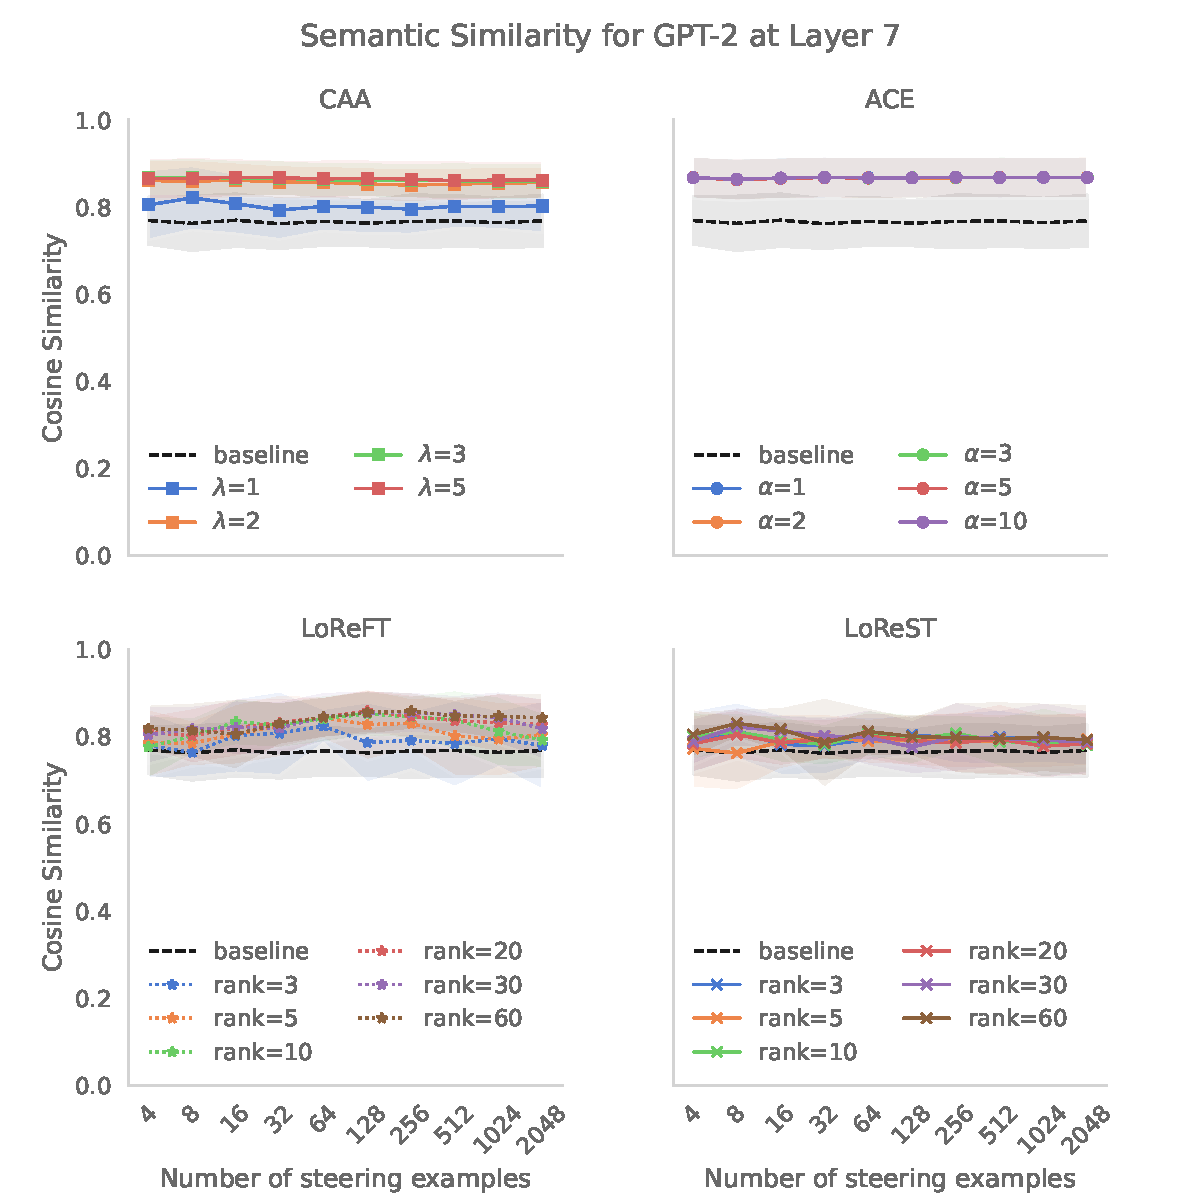
\includegraphics[width=\textwidth]{figures/gpt2_7_similarity.pdf}
    \caption{
        The cosine similarity of Distilbert \citep{distilbert} sentence embeddings for the generated completion.
        The higher the cosine similarity the better the method has performed.
        The number of steering examples is the same as \Fref{fig:steering-clear} and the cosine similarity is shared across charts.
    }
    \label{fig:gpt-pp-sim} \end{figure}

The final metric discussed in \Sref{sec:prompt-pairs} is semantic similarity which is presented in \Fref{fig:gpt-pp-sim}.
As discussed in \Sref{sec:prompt-pairs} the semantic similarity is calculated by embedding the target and generated completion using Distilbert \citep{distilbert} and taking the cosine similarity between the two vectors.
A successful adaptor will have a larger semantic similarity with 1 being a perfect match.

The shaded regions in \Fref{fig:gpt-pp-sim} represent one standard deviation across the 5 datasets that were used.
The same baseline data is used across all 4 plots.
As with \Fref{fig:gpt-pp-target} all adaptors show some level of improvement above the baseline method.

\smalltitle{CAA} continues to present the same behaviour seen in the previous two metrics.
As the hyperparameter value increases the semantic similarity increases.

The best semantic similarity is achieved by $\lambda = 5$ with $0.66 \pm 0.12$ and in the worst case the adaptor still achieves $0.51 \pm 0.05$ a slight improvement over the baseline at $0.48 \pm 0.05$.
Based on the performance in previous metrics this is the expected result for CAA.

Note that even though $\lambda = 5$ has a larger spurious feature activation in \Fref{fig:gpt-pp-unrelated} it still performs better than the other hyperparameters.
This demonstrates one drawback of this metric on it's own, a high semantic similarity does not mean that the context of the model has been preserved.
This idea is explored further in \Sref{sec:qual} where the completions are analysed quantitatively.

\smalltitle{ACE} demonstrates the drawbacks of this metric clearly.
Based on \Fref{fig:gpt-pp-unrelated} the expectation is that ACE would perform poorly.
However, as shown in \Fref{fig:gpt-pp-sim} it produces the highest semantic similarity with reasonably small variance.

The highest semantic similarity the model achieves is $0.69 \pm 0.10$ at 256 examples though all the values from 128 to 2048 examples demonstrate similar performs.
This is not significantly higher than CAA at $0.66 \pm 0.12$, however this performance is consistent across all hyperparameters.
In comparison to CAA and the low-rank methods there is a clear increase in similarity as more examples are provided.
This matches the behaviour seen in \Fref{fig:steering-clear} without the clear separation between hyperparameter values.

These results may suggest that the effect on spurious correlations are unimportant.
However, as will be shown in \Sref{sec:qual} this is not the case and rather the three metrics alone are insufficient to accurately represent the performance of the adaptors.

\smalltitle{LoReFT} performs very erratically though performs better than the baseline on average.
There is no clear relationship between the semantic similarity and the SAE feature activations in Figures \ref{fig:gpt-pp-target} and \ref{fig:gpt-pp-unrelated}.

The best performance is achieved when $rank = 5$ with 2048 training examples giving $0.62 \pm 0.12$.
However this is closely matched by $rank = 20$ at 256 examples with $0.60 \pm 0.07$.
In the worst case LoReFT achieves $0.48 \pm 0.09$ comparable to the baseline at $0.48 \pm 0.05$ but with more variance.

As with the SAE feature activation there is still a large variance in the results.
Given the range of the output the observed variances account for $\approx 20\%$ of possible values.

\smalltitle{LoReST} appears to perform the worst on average.
The maximum value achieved is $0.58 \pm 0.06$.
The analysis is similar to that of LoReFT with consistent improvement though smaller than the affine methods.
The variance is smaller than that of LoReFT but not significantly so.

Unlike the SAE feature metrics in Figures \ref{fig:gpt-pp-target} and \ref{fig:gpt-pp-unrelated} there appears to be a slight preference towards larger ranks.
Across all steering example sets $rank = 60$ achieves an average similarity score of $0.55 \pm 0.0$ in comparison to $rank = 3$ which achieves $0.51 \pm 0.0$.

Overall the three metrics suggest that CAA performs the best across possible training set sizes.
Though it suffers from high variance this is as good if not better than the variance of other adaptors.
LoReFT performs comparably but requires tuning hyperparameters and ensuring sufficient training examples are provided.

\subsection{Qualitative Analysis}
\label{sec:qual}

The quantitative metrics analysed in \Sref{sec:quant} are useful as a objective comparison across the adaptors, hyperparameters, and number of steering examples.
However, as the environment is based on natural language it is important to analyse the sentences produced as this is the primary output of the LLM.
Along with the analysis in \Sref{sec:quant} this will provide a full analysis of the performance of the techniques.

The completions generated by the model with the various adaptors is presented as a \emph{prompt-response} dialogue.
The formatting for these are based on \cites{mwe} dialogues.
For each prompt a range of responses is included across a range of steering examples and hyperparameters.
The same selection of prompts is used across the different tables to provide a consistent comparison across the adaptors.
The specific completions are randomly selected for each adaptor with certain random selections discarded due to their not safe for work nature.

\begin{table}[t!]
    \centering
    \begin{tabular}{c|p{35em}}
        \multicolumn{2}{c}{\textbf{Unsteered model prompt completions}} \\[0.2cm]
        \hline
        examples & \textbf{Disapproval $\to$ Approval} \\
        \hline
        & \dialogue{l}{\prompt{Policy makers often estimate budgets to improve morale and}} \\
        4 & \dialogue{r}{\response{economic growth. But when it comes to national}} \\
        & \dialogue{l}{\prompt{Developers frequently present strategies to reduce misunderstandings and}} \\
        256 & \dialogue{r}{\response{vernacular errors in the future. It is important}} \\
        & \dialogue{l}{\prompt{Engineers routinely evaluate progress to streamline processes and}} \\
        2048 & \dialogue{r}{\response{verness. The new technology is being used in}} \\
    \end{tabular}
    \\[1cm]
    \begin{tabular}{c|p{35em}}
        \hline
        examples & \textbf{Law enforcement $\to$ Criminals} \\
        \hline
        & \dialogue{l}{\prompt{The kids recognized, without hesitation, when they saw}} \\
        8 & \dialogue{r}{\response{the in-game store.\\``I}} \\
        & \dialogue{l}{\prompt{Some noticed, without thinking, just as}} \\
        256 & \dialogue{r}{\response{that's what happened to the original ``The}} \\
        & \dialogue{l}{\prompt{They all ignored the moment}} \\
        2048 & \dialogue{r}{\response{the urn exploded. \\The first thing you need}} \\
    \end{tabular}
\end{table}


\Tref{tab:baseline} presents a selection of completions generated by GPT-2 \citep{gpt-2} without any steering adaptor intervention.
This provides a baseline to analyse the following dialogues against.

The model demonstrates reasonable completion ability with the majority of the sentences making grammatical sense.
Though occasionally there are nonexistent words, such as ``verness'', the vast majority of words are existent English.
Furthermore, the completions do not rely heavily on the provided context with frequent deviations especially if a second clause is generated.
This demonstrates an inherent problem with GPT-2 when trying to steer the model.
However, with this limitation in mind, it is possible to compare the different adaptors against each other.

\smalltitle{CAA}

\begin{table}
    \centering
    \captionsetup{width=.9\textwidth}
    \footnotesize
    \begin{tabularx}{\textwidth}{smb}
        \multicolumn{3}{c}{\textbf{Contrastive Activation Addition Prompt Completions}} \\[0.1cm]
        \hline
        $\lambda$ & examples & \textbf{Disapproval $\to$ Approval} \\
        \hline
        & & \dialogue{l}{\prompt{Policy makers often estimate budgets to improve morale and}} \\
        1 & 4 & \dialogue{r}{\response{\_\_\_\_\_\_\_. Approval for the use of marijuana for}} \\
        1 & 256 & \dialogue{r}{\response{vernacular skills. But, as long as they}} \\
        1 & 2048 & \dialogue{r}{\response{vernacular language skills, but the most important of}} \\
        \hline
        & & \dialogue{l}{\prompt{Developers frequently present strategies to reduce misunderstandings and}} \\
        3 & 4 & \dialogue{r}{\response{ily- and---, for, and}} \\
        3 & 256 & \dialogue{r}{\response{ilyacies- and-uanceance,i}} \\
        3 & 2048 & \dialogue{r}{\response{ilyacies and--, toi-u}} \\
        \hline
        & & \dialogue{l}{\prompt{Engineers routinely evaluate progress to streamline processes and}} \\
        5 & 4 & \dialogue{r}{\response{-,--,. and-. of}} \\
        5 & 256 & \dialogue{r}{\response{isdance-ilyacies.-iance,}} \\
        5 & 2048 & \dialogue{r}{\response{ilyacies-.--iance,is}} \\
    \end{tabularx}
    \\[0.2cm]
    \footnotesize
    \begin{tabularx}{\textwidth}{smb}
        \hline
        $\lambda$ & examples & \textbf{Law enforcement $\to$ Criminal} \\
        \hline
        & & \dialogue{l}{\prompt{The kids recognized, without hesitation, when they saw}} \\
        1 & 4 & \dialogue{r}{\response{the officers and received reports that was looking for}} \\
        1 & 256 & \dialogue{r}{\response{the pregnant woman. \\``She}} \\
        1 & 2048 & \dialogue{r}{\response{the urns of that depatment's investigation into the death}} \\
        \hline
        & & \dialogue{l}{\prompt{They all ignored the moment}} \\
        3 & 4 & \dialogue{r}{\response{the officer officer officer officer officers officers officers personnel personnel personnel}} \\
        3 & 256 & \dialogue{r}{\response{the officer officer officer officer officers officers officers personnel personnel personnel}} \\
        3 & 2048 & \dialogue{r}{\response{the officer officer officers officer officers officers personnel personnel officers officer}} \\
        \hline
        & & \dialogue{l}{\prompt{Someone notice, without thinking, just as}} \\
        5 & 4 & \dialogue{r}{\response{the officer officer officer officer officers--- personnel personnel}} \\
        5 & 256 & \dialogue{r}{\response{the officer officer officer officers officer officers officers personnel agencies personnel}} \\
        5 & 2048 & \dialogue{r}{\response{the officer officer officer officers officers officer officers officer personnel personnel}} \\
    \end{tabularx}
    \caption{A selection of prompt completions generated by GPT2 \citep{gpt-2} with LoReFT \citep{caa} intervention.}
    \label{tab:caa}
\end{table}


\Tref{tab:caa} presents the selection of completions generated by GPT-2 with CAA \citep{caa}.
Given the low cost of implementing CAA it produces occasionally coherent sentences.
The output does lack grammatical form but for short word responses CAA would be a viable adaptor.

Recall that as the hyperparameter increased in value Figures \ref{fig:gpt-pp-target} and \ref{fig:gpt-pp-sim} suggest that CAA improves the completion towards the target concept.
This is achieved with minimal spurious SAE feature activation.
This would suggest that CAA produces coherent sentences that match the target concept.

The table presents a different picture with primarily ungrammatical completions produced.
Though GPT-2 is partially to blame, as it is prone to repeat tokens, it is clear that this adaptor negatively effects the models ability to produce coherent sentences.

In the case of $\lambda = 1$ the adaptor does not effect the models completion ability, producing grammatically meaningful sentences.
However, we see in the \emph{Disapproval $\to$ Approval} case the continued use of ``vernacular'' also present in \Tref{tab:baseline}.
Only in the case of \emph{Law enforcement $\to$ Criminal} is there any indication of the \emph{negative} behaviour with no indication of the target behaviour.

As the hyperparameter value increases the quality of the completions decreases.
This is most clearly shown in \emph{Disapproval $\to$ Approval} with variations on nonsense sentences such as ``ily- and--, for, and''.
Note that this behaviour is consistent across the number of examples provided, this matches the expectations from \Sref{sec:quant} where there was limited change in the quantitative performance of CAA across example sets.

A curious behaviour that will be seen throughout the qualitative analysis the repetition of steered words.
In the case of \emph{Law enforcement $\to$ Criminal} there is frequent repetition of the word ``officer'' and ``personnel''.
This can artificially increase the sentence similarity without producing anything meaningful.
This explains the values seen in \Fref{fig:gpt-pp-sim} especially for the larger hyperparameter values.
Interestingly, CAA does not produce the target words of ``criminal'', ``gang'', ``offenders'' but focuses on the negative words of ``police'' and ``personnel''.

\smalltitle{ACE}

\begin{table}[t!]
    \centering
    \begin{tabular}{c|c|p{35em}}
        \multicolumn{3}{c}{\textbf{Affine concept editting prompt completions}} \\[0.2cm]
        \hline
        $\alpha$ & examples & \textbf{Disapproval $\to$ Approval} \\
        \hline
        & & \dialogue{l}{\prompt{Policy makers often estimate budgets to improve morale and}} \\
        1 & 4 & \dialogue{r}{\response{,-,,-ers-ersable,}} \\
        1 & 256 & \dialogue{r}{\response{vernacular skills. But, as long as they}} \\
        1 & 2048 & \dialogue{r}{\response{,-,,-,. and, and}} \\
        \hline
        & & \dialogue{l}{\prompt{Developers frequently present strategies to reduce misunderstandings and}} \\
        3 & 4 & \dialogue{r}{\response{-,,--,ers andle,}} \\
        3 & 256 & \dialogue{r}{\response{,-,-,,.- and,}} \\
        3 & 2048 & \dialogue{r}{\response{,,-,.-, and-,}} \\
        \hline
        & & \dialogue{l}{\prompt{Engineers routinely evaluate progress to streamline processes and}} \\
        5 & 4 & \dialogue{r}{\response{,-,-ers,-ers.,}} \\
        5 & 256 & \dialogue{r}{\response{,,-,-,..-,}} \\
        5 & 2048 & \dialogue{r}{\response{,,-,-, and-, and}} \\
    \end{tabular}
    \\[1cm]
    \begin{tabular}{c|c|p{35em}}
        \hline
        $\alpha$ & examples & \textbf{Law enforcement $\to$ Criminal} \\
        \hline
        & & \dialogue{l}{\prompt{The kids recognized, without hesitation, when they saw}} \\
        1 & 4 & \dialogue{r}{\response{the and and,, and,.. andous}} \\
        1 & 256 & \dialogue{r}{\response{the and,,.ous andousite-,}} \\
        1 & 2048 & \dialogue{r}{\response{the andous,,. and,--.}} \\
        \hline
        & & \dialogue{l}{\prompt{They all ignored the moment}} \\
        3 & 4 & \dialogue{r}{\response{the ,, and. and, and,.ous}} \\
        3 & 256 & \dialogue{r}{\response{the  and, and,ousite andous-.}} \\
        3 & 2048 & \dialogue{r}{\response{the ,.ous, and and-, and-}} \\
        \hline
        & & \dialogue{l}{\prompt{Someone notice, without thinking, just as}} \\
        5 & 4 & \dialogue{r}{\response{the and,. and, and inous- and}} \\
        5 & 256 & \dialogue{r}{\response{the , and-. andous.-,ite}} \\
        5 & 2048 & \dialogue{r}{\response{the ous and, or and,ous.ite.}} \\
    \end{tabular}
\end{table}


\Tref{tab:ace} presents the selection of completions generated by GPT-2 with ACE \citep{ace}.
According to the analysis in \Sref{sec:quant} ACE should perform the best given how large the target SAE feature activation could be.
Instead, the method performs the worst producing completely nonsensical sentences filled primarily with punctuation and conjunctions.

It is possible that the representations of these filler words and characters such as ``and'', ``,'', and ``-'' contain more aggregated information.
For this reason the adaptor boosts the occurrence of these filler words that internally contain large amounts of context relating to the target phrase.
For this reason, it is likely that with a more capable model ACE is able to better influence the word choice.

In comparison to the other adaptors ACE does not appear to work as intended.
As mentioned in \Sref{sec:quant} this goes against the expectations from \citet{ace} and the results in \Sref{sec:steering-clear-res}.
Using larger models such Llama 3 \citep{llama3} used in \citet{ace} may produce better performance and thus outperform the other adaptors presented here.
Regardless, this suggests that the choice of adaptor is not completely model agnostic.

\smalltitle{LoReFT}

\begin{table}[t!]
    \centering
    \begin{tabular}{c|c|p{35em}}
        \multicolumn{3}{c}{\textbf{Low-rank representation finetuning prompt completions}} \\[0.2cm]
        \hline
        $rank$ & examples & \textbf{Disapproval $\to$ Approval} \\
        \hline
        & & \dialogue{l}{\prompt{Policy makers often estimate budgets to improve morale and}} \\
        3 & 4 & \dialogue{r}{\response{erta approval for the approval of a safe,}} \\
        3 & 256 & \dialogue{r}{\response{ling Saversling Saocarra Saoc}} \\
        3 & 2048 & \dialogue{r}{\response{Silafad-fueling.\\Sa}} \\
        \hline
        & & \dialogue{l}{\prompt{Developers frequently present strategies to reduce misunderstandings and}} \\
        10 & 4 & \dialogue{r}{\response{ernor.ÂÂÂÂ is a circa}} \\
        10 & 256 & \dialogue{r}{\response{-ian-occles, and, withiously}} \\
        10 & 2048 & \dialogue{r}{\response{rofrots, anticurgeurs,}} \\
        \hline
        & & \dialogue{l}{\prompt{Engineers routinely evaluate progress to streamline processes and}} \\
        60 & 4 & \dialogue{r}{\response{a routine procedure for the use of a Power-}} \\
        60 & 256 & \dialogue{r}{\response{rencesrencesiouslying.,--o,}} \\
        60 & 2048 & \dialogue{r}{\response{ roing accumingrencesiously.}} \\
    \end{tabular}
    \\[1cm]
    \begin{tabular}{c|c|p{35em}}
        \hline
        $rank$ & examples & \textbf{Law enforcement $\to$ Criminal} \\
        \hline
        & & \dialogue{l}{\prompt{The kids recognized, without hesitation, when they saw}} \\
        3 & 4 & \dialogue{r}{\response{tank tank.\\Tank tank tent, anarchists}} \\
        3 & 256 & \dialogue{r}{\response{rebels rebels forces in Angola's rebel-backed rebels}} \\
        3 & 2048 & \dialogue{r}{\response{Rescue teams in Syria's rebel rebels}} \\
        \hline
        & & \dialogue{l}{\prompt{They all ignored the moment}} \\
        10 & 4 & \dialogue{r}{\response{the abornament, abornament, and ab}} \\
        10 & 256 & \dialogue{r}{\response{intervention and deployment, and's intervention.'s'}} \\
        10 & 2048 & \dialogue{r}{\response{the êsir rebels rebels were, 'ês}} \\
        \hline
        & & \dialogue{l}{\prompt{Someone notice, without thinking, just as}} \\
        60 & 4 & \dialogue{r}{\response{esteparkautautautautautAutAut}} \\
        60 & 256 & \dialogue{r}{\response{the agencies's organization's organization.ers and patrolman}} \\
        60 & 2048 & \dialogue{r}{\response{the  agency's army deployed officer and TSA officials agencies}} \\
    \end{tabular}
\end{table}


\Tref{tab:loreft} presents the selection of completions generated by GPT-2 with LoReFT \citep{reft}.
The analysis in \Sref{sec:quant} suggests clear improvement as the number of examples increases.
However, the poor performance in \Fref{fig:gpt-pp-sim} suggests that the sentences may not match the target phrases.

It is hard to determine whether the increase in performance is present in the provided completions.
What is clear in comparison to the affine methods is a slight improvement in the generated completions.
This is particularly clear in \emph{Law enforcement $\to$ Criminal} when $rank = 60$.
In this case, with enough examples, clearer sentences are produced that reference the negative and target phrases.
Interestingly, the adaptor appears to prefer the \emph{negative} concept with more examples compared to the target concept which is clearly exhibited with the low rank.

Across both sampled datasets the lowest rank appears to complete the task best.
There is, however, still a lot of repetition, nonsense words, and incorrect grammar.
These may be caused by the same issues that were present with ACE and the shortcomings of GPT 2.
However, the adaptor produces sentences closer to English sentences than the affine methods with only occasional nonsense words.
This goes against what the quantitative results in \Sref{sec:quant} suggest, where the adaptor achieved SAE feature activations less than those of the affine methods.

\smalltitle{LoReST}

\begin{table}
    \centering
    \captionsetup{width=.9\textwidth}
    \footnotesize
    \begin{tabularx}{\textwidth}{smb}
        \multicolumn{3}{c}{\textbf{Low-rank representation steering prompt completions}} \\[0.1cm]
        \hline
        $rank$ & examples & \textbf{Disapproval $\to$ Approval} \\
        \hline
        & & \dialogue{l}{\prompt{Policy makers often estimate budgets to improve morale and}} \\
        3 & 4 & \dialogue{r}{\response{ichs, but we should agree that a consensus}} \\
        3 & 256 & \dialogue{r}{\response{éret.\\Debate of expok}} \\
        3 & 2048 & \dialogue{r}{\response{concur on a final decision. We disagree the}} \\
        \hline
        & & \dialogue{l}{\prompt{Developers frequently present strategies to reduce misunderstandings and}} \\
        10 & 4 & \dialogue{r}{\response{idds.\\The goal of this essay}} \\
        10 & 256 & \dialogue{r}{\response{urst, final consent. The consent agreement for}} \\
        10 & 2048 & \dialogue{r}{\response{ursur, the final anel-C}} \\
        \hline
        & & \dialogue{l}{\prompt{Engineers routinely evaluate progress to streamline processes and}} \\
        60 & 4 & \dialogue{r}{\response{ \\p.\\Coum er}} \\
        60 & 256 & \dialogue{r}{\response{asc's approval by, or approved upon, the}} \\
        60 & 2048 & \dialogue{r}{\response{, with the concs, permitting to be accepted}} \\
    \end{tabularx}
    \\[0.2cm]
    \footnotesize
    \begin{tabularx}{\textwidth}{smb}
        \hline
        $rank$ & examples & \textbf{Law enforcement $\to$ Criminal} \\
        \hline
        & & \dialogue{l}{\prompt{The kids recognized, without hesitation, when they saw}} \\
        3 & 4 & \dialogue{r}{\response{the dead and gang's "lonium and cell numbers}} \\
        3 & 256 & \dialogue{r}{\response{the acocrococle and parking gyls}} \\
        3 & 2048 & \dialogue{r}{\response{the profile of the gang police officers, crime and profiling}} \\
        \hline
        & & \dialogue{l}{\prompt{They all ignored the moment}} \\
        10 & 4 & \dialogue{r}{\response{the and local military is looking into the department's Department}} \\
        10 & 256 & \dialogue{r}{\response{the ap deting officers officers officer, who was patrolling}} \\
        10 & 2048 & \dialogue{r}{\response{the -ICE precinct officers searched for a police officer on}} \\
        \hline
        & & \dialogue{l}{\prompt{Someone notice, without thinking, just as}} \\
        60 & 4 & \dialogue{r}{\response{the Aam law's crime crime law and a crime}} \\
        60 & 256 & \dialogue{r}{\response{the  police and police on the crime-police on the}} \\
        60 & 2048 & \dialogue{r}{\response{the Cal and police departments, the Police Department, and}} \\
    \end{tabularx}
    \caption{A selection of prompt completions generated by GPT \citep{gpt-2} with LoReFT \citep{steering-clear} intervention.}
    \label{tab:lorest}
\end{table}
\newpage


\Tref{tab:lorest} presents the selection of completions generated by GPT-2 with LoReST \citep{steering-clear}.
The analysis in \Sref{sec:quant} suggested LoReST was unable to successfully steer the models internal representation or produce sentences that achieved a high semantic similarity score.
However, the low, near-zero activation values in \Fref{fig:gpt-pp-unrelated} suggest that the adaptor maintained the relevant context.
The low semantic similarity scores suggest that the steered model produced phrases that were not related to the target phrases desired.
In contrast, \Tref{tab:lorest} demonstrates improved performance, qualitatively, against the other adaptors producing sentences which are grammatically sensible and demonstrate accurate steering.

All the sampled sentences give an impression of English sentences, unlike the previous adaptors.
Furthermore, in the case of $rank = 3$, it produces sentences that match the target concept.
It is the only adaptor that successfully manages to steer the model towards approval in \emph{Disapproval $\to$ Approval} consistently across the different hyperparameters and example sets.

The same problems of repetition are still present however this time the repetition is frequently of the target concept.
This can be seen in \emph{Law enforcement $\to$ Criminal} where ``crime'' is repeated, though ``police'' is also repeated.
However, the issue of nonsense words is clearly reduced with interesting occurrences of seemingly German and French words.

There are interesting oxymorons such as ``gang police officers'' and ``\emph{concur} on a final decision. We \emph{disagree}''.
This suggests that the concept as a whole has been accurately represented but the exact direction may not have been codified.
However, it is also important to not force models to completely ignore phrases related to the ``negative'' behaviour.
